\chapter{Varroa Execution}

Varroa has two main modes of execution for now. One is to configure Varroa ahead of time manually or programmatically and then execute directly. The other is to use containers and utilize dynamic discovery.

\section{Configuration}
Following are the two sequence sketches for direct (static initialization) configuration \ref{pic:staticExecution} and dynamic (DNS discovery based) \ref{pic:dynamicExecution} configuration.

\section{Static configuration}
\begin{figure}[h]
\begin{center}
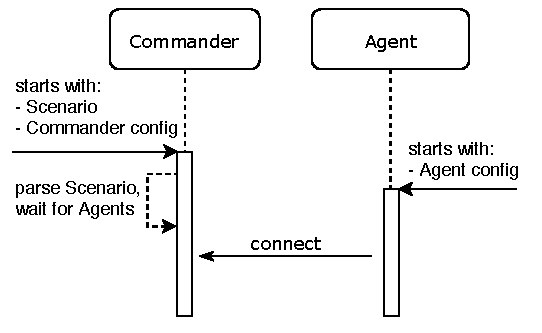
\includegraphics[scale=0.65]{Resources/PDF/ExecutionStaticInit}
\caption{static execution}
\label{pic:staticExecution}
\end{center}
\end{figure}

Static configuration may be used on any infrastructure where hostname or ip addresses of all Varroa instances (commander and agents) are known ahead of time. This is the case on most typical systems, such as IaaS clouds where an instance is booted and assigned an address before the application is deployed onto that system.

For static configuration, the user must provide an instance configuration, which configures the Varroa instance as a commander or an agent (or possibly both), as well as (optionally) the instance limits specifying how much load the agent can generate.

\lstset{language=xml}

\begin{figure}

\begin{lstlisting}[frame=single]
<varroa>
    <commander>
        <bind-port>12345</bind-port>
        <amount-agents>3</amount-agents>
    </commander>
</varroa>
\end{lstlisting}
\caption{A sample static commander configuration}
\end{figure}
\section{Dynamic configuration}

\begin{figure}[h]
\begin{center}
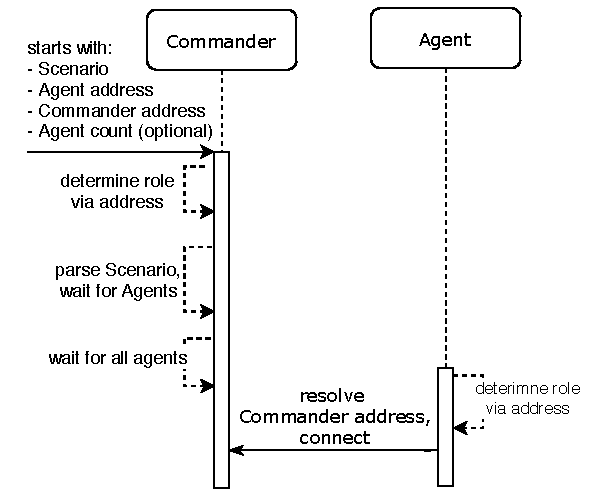
\includegraphics[scale=0.65]{Resources/PDF/ExecutionDnsInit}
\caption{dynamic execution}
\label{pic:dynamicExecution}
\end{center}
\end{figure}

DNS discovery specifically is aimed at container environments and cloud platforms. These types of platforms generally provide different methods of service discovery, which are necessary to allow the parts of a distributed systems to communicate with each other.

In container environments especially, the address of a server an application is going to run on is generally not known ahead of application startup. Containers are launched quickly and in an unpredictable order, leading to a scenario where the addresses of all parts of a system cannot be known ahead of time. This necessitates a configuration method which allows service discovery after application startup, which the previous method cannot handle.

Dynamic configuration allows Varroa to start without knowing the addresses of any other Varroa instances nor its own role. The way the initial DNS discovery method works is by supplying hostnames for the commander and agent groups respectively.


\begin{figure}[h]
\begin{center}
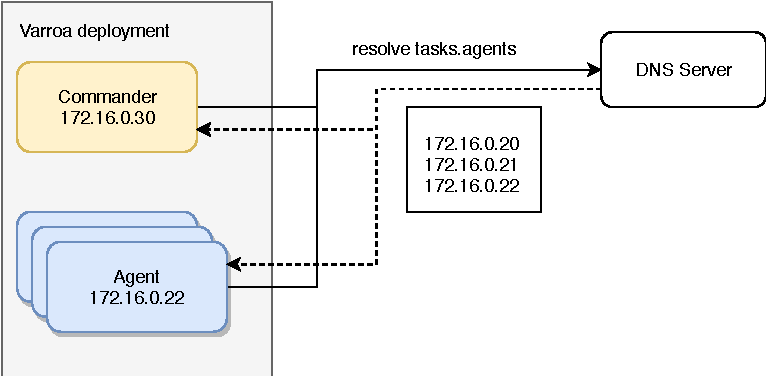
\includegraphics[scale=0.65]{Resources/PDF/ExecutionDnsDiscovery}
\caption{agent record resolution}
\end{center}
\end{figure}

At startup Varroa will continuously resolve those records, which must be a round-robin A record, and compare each address found in the records to the address corresponding to its own hostname. If any address matches its own, the instance will set its role according to the set of addresses it matches.

Additionally, agents can use the commander address to locate the commander node and continuously attempt to connect to it until it is ready for agent connections.

The commander can also determine how many agents will connect to it using the agent address, or alternatively a agent count can be  provided at startup (for deployments on services where records are slowly updated as containers start).

\begin{figure}
\begin{lstlisting}
VARROA_DNS_AGENT=tasks.agents
VARROA_DNS_COMMANDER=tasks.commander
VARROA_DNS_AGENT_COUNT=3
\end{lstlisting}
\caption{A sample dynamic discovery configuration, showing the environment variable values}
\end{figure}